\documentclass[twoside]{book}

% Packages required by doxygen
\usepackage{fixltx2e}
\usepackage{calc}
\usepackage{doxygen}
\usepackage[export]{adjustbox} % also loads graphicx
\usepackage{graphicx}
\usepackage[utf8]{inputenc}
\usepackage{makeidx}
\usepackage{multicol}
\usepackage{multirow}
\PassOptionsToPackage{warn}{textcomp}
\usepackage{textcomp}
\usepackage[nointegrals]{wasysym}
\usepackage[table]{xcolor}

% Font selection
\usepackage[T1]{fontenc}
\usepackage[scaled=.90]{helvet}
\usepackage{courier}
\usepackage{amssymb}
\usepackage{sectsty}
\renewcommand{\familydefault}{\sfdefault}
\allsectionsfont{%
  \fontseries{bc}\selectfont%
  \color{darkgray}%
}
\renewcommand{\DoxyLabelFont}{%
  \fontseries{bc}\selectfont%
  \color{darkgray}%
}
\newcommand{\+}{\discretionary{\mbox{\scriptsize$\hookleftarrow$}}{}{}}

% Page & text layout
\usepackage{geometry}
\geometry{%
  a4paper,%
  top=2.5cm,%
  bottom=2.5cm,%
  left=2.5cm,%
  right=2.5cm%
}
\tolerance=750
\hfuzz=15pt
\hbadness=750
\setlength{\emergencystretch}{15pt}
\setlength{\parindent}{0cm}
\setlength{\parskip}{3ex plus 2ex minus 2ex}
\makeatletter
\renewcommand{\paragraph}{%
  \@startsection{paragraph}{4}{0ex}{-1.0ex}{1.0ex}{%
    \normalfont\normalsize\bfseries\SS@parafont%
  }%
}
\renewcommand{\subparagraph}{%
  \@startsection{subparagraph}{5}{0ex}{-1.0ex}{1.0ex}{%
    \normalfont\normalsize\bfseries\SS@subparafont%
  }%
}
\makeatother

% Headers & footers
\usepackage{fancyhdr}
\pagestyle{fancyplain}
\fancyhead[LE]{\fancyplain{}{\bfseries\thepage}}
\fancyhead[CE]{\fancyplain{}{}}
\fancyhead[RE]{\fancyplain{}{\bfseries\leftmark}}
\fancyhead[LO]{\fancyplain{}{\bfseries\rightmark}}
\fancyhead[CO]{\fancyplain{}{}}
\fancyhead[RO]{\fancyplain{}{\bfseries\thepage}}
\fancyfoot[LE]{\fancyplain{}{}}
\fancyfoot[CE]{\fancyplain{}{}}
\fancyfoot[RE]{\fancyplain{}{\bfseries\scriptsize Generated by Doxygen }}
\fancyfoot[LO]{\fancyplain{}{\bfseries\scriptsize Generated by Doxygen }}
\fancyfoot[CO]{\fancyplain{}{}}
\fancyfoot[RO]{\fancyplain{}{}}
\renewcommand{\footrulewidth}{0.4pt}
\renewcommand{\chaptermark}[1]{%
  \markboth{#1}{}%
}
\renewcommand{\sectionmark}[1]{%
  \markright{\thesection\ #1}%
}

% Indices & bibliography
\usepackage{natbib}
\usepackage[titles]{tocloft}
\setcounter{tocdepth}{3}
\setcounter{secnumdepth}{5}
\makeindex

% Hyperlinks (required, but should be loaded last)
\usepackage{ifpdf}
\ifpdf
  \usepackage[pdftex,pagebackref=true]{hyperref}
\else
  \usepackage[ps2pdf,pagebackref=true]{hyperref}
\fi
\hypersetup{%
  colorlinks=true,%
  linkcolor=blue,%
  citecolor=blue,%
  unicode%
}

% Custom commands
\newcommand{\clearemptydoublepage}{%
  \newpage{\pagestyle{empty}\cleardoublepage}%
}

\usepackage{caption}
\captionsetup{labelsep=space,justification=centering,font={bf},singlelinecheck=off,skip=4pt,position=top}

%===== C O N T E N T S =====

\begin{document}

% Titlepage & ToC
\hypersetup{pageanchor=false,
             bookmarksnumbered=true,
             pdfencoding=unicode
            }
\pagenumbering{alph}
\begin{titlepage}
\vspace*{7cm}
\begin{center}%
{\Large C\+O\+P290 }\\
\vspace*{1cm}
{\large Generated by Doxygen 1.8.14}\\
\end{center}
\end{titlepage}
\clearemptydoublepage
\pagenumbering{roman}
\tableofcontents
\clearemptydoublepage
\pagenumbering{arabic}
\hypersetup{pageanchor=true}

%--- Begin generated contents ---
\chapter{C\+O\+P290}
\label{md__r_e_a_d_m_e}
\Hypertarget{md__r_e_a_d_m_e}
\section*{E\+D\+Tool \+:}

This repository holds the assignment allotted as a part of course C\+O\+P290(design practices), I\+IT Delhi. It is used to make a 3D object from it\textquotesingle{}s orthographic projections and projection of 3D object on a plane.

\section*{Aim \+:}

The package has following functionalities \+:
\begin{DoxyEnumerate}
\item Able to interactively input or read from a file either i) an isometric drawing and a 3D object model or ii) projections on to any cross section.
\item Given the 3D model description we should be able to generate projections on to any cross section or cutting plane.
\item Given two or more projections we should be able to interactively recover the 3D description and produce an isometric drawing from any view direction.
\end{DoxyEnumerate}

\section*{Organisation of the code \+:}

Following is the description of the directories\+:

\section*{G\+T\+K\+MM \+:}

The project makes use of the G\+T\+Kmm libraries for C++. Hence this package is needed to be installed before running the software package. Use the following command\+: 
\begin{DoxyCode}
sudo apt-get install libgtkmm-3.0-dev
\end{DoxyCode}
 The above command installs the requisite packages. Now the software package can be built and used.

\section*{Compilation and execution instructions \+:}

Enter the project directory and run the following command 
\begin{DoxyCode}
make
\end{DoxyCode}
 Then cd into the build folder and run the following 
\begin{DoxyCode}
./main
\end{DoxyCode}


\section*{Assumptions \+:}

Given in the design document.

\section*{Things that has been deleted/changed since the last submission \+:}

Some of the functions have been deleted and incorporated in the main file. Files like hidden.\+cpp have been combined with the code and the structure of individual classes and header files have been somewhat changed on the suggestion of TA and the professor. New features like the hidden lines that have been mentioned in design document have been built upon and executed. 
\chapter{Hierarchical Index}
\section{Class Hierarchy}
This inheritance list is sorted roughly, but not completely, alphabetically\+:\begin{DoxyCompactList}
\item Drawing\+Area\begin{DoxyCompactList}
\item \contentsline{section}{My\+Area}{\pageref{class_my_area}}{}
\item \contentsline{section}{My\+Area1}{\pageref{class_my_area1}}{}
\end{DoxyCompactList}
\item \contentsline{section}{home}{\pageref{classhome}}{}
\item \contentsline{section}{vertex}{\pageref{classvertex}}{}
\item Window\begin{DoxyCompactList}
\item \contentsline{section}{Main}{\pageref{class_main}}{}
\item \contentsline{section}{Three2}{\pageref{class_three2}}{}
\item \contentsline{section}{Two3}{\pageref{class_two3}}{}
\end{DoxyCompactList}
\end{DoxyCompactList}

\chapter{Class Index}
\section{Class List}
Here are the classes, structs, unions and interfaces with brief descriptions\+:\begin{DoxyCompactList}
\item\contentsline{section}{\mbox{\hyperlink{classhome}{home}} }{\pageref{classhome}}{}
\item\contentsline{section}{\mbox{\hyperlink{class_main}{Main}} }{\pageref{class_main}}{}
\item\contentsline{section}{\mbox{\hyperlink{class_my_area}{My\+Area}} }{\pageref{class_my_area}}{}
\item\contentsline{section}{\mbox{\hyperlink{class_my_area1}{My\+Area1}} }{\pageref{class_my_area1}}{}
\item\contentsline{section}{\mbox{\hyperlink{class_three2}{Three2}} }{\pageref{class_three2}}{}
\item\contentsline{section}{\mbox{\hyperlink{class_two3}{Two3}} }{\pageref{class_two3}}{}
\item\contentsline{section}{\mbox{\hyperlink{classvertex}{vertex}} }{\pageref{classvertex}}{}
\end{DoxyCompactList}

\chapter{Class Documentation}
\hypertarget{classhome}{}\section{home Class Reference}
\label{classhome}\index{home@{home}}


The documentation for this class was generated from the following file\+:\begin{DoxyCompactItemize}
\item 
src/main.\+cpp\end{DoxyCompactItemize}

\hypertarget{class_main}{}\section{Main Class Reference}
\label{class_main}\index{Main@{Main}}
Inheritance diagram for Main\+:\begin{figure}[H]
\begin{center}
\leavevmode
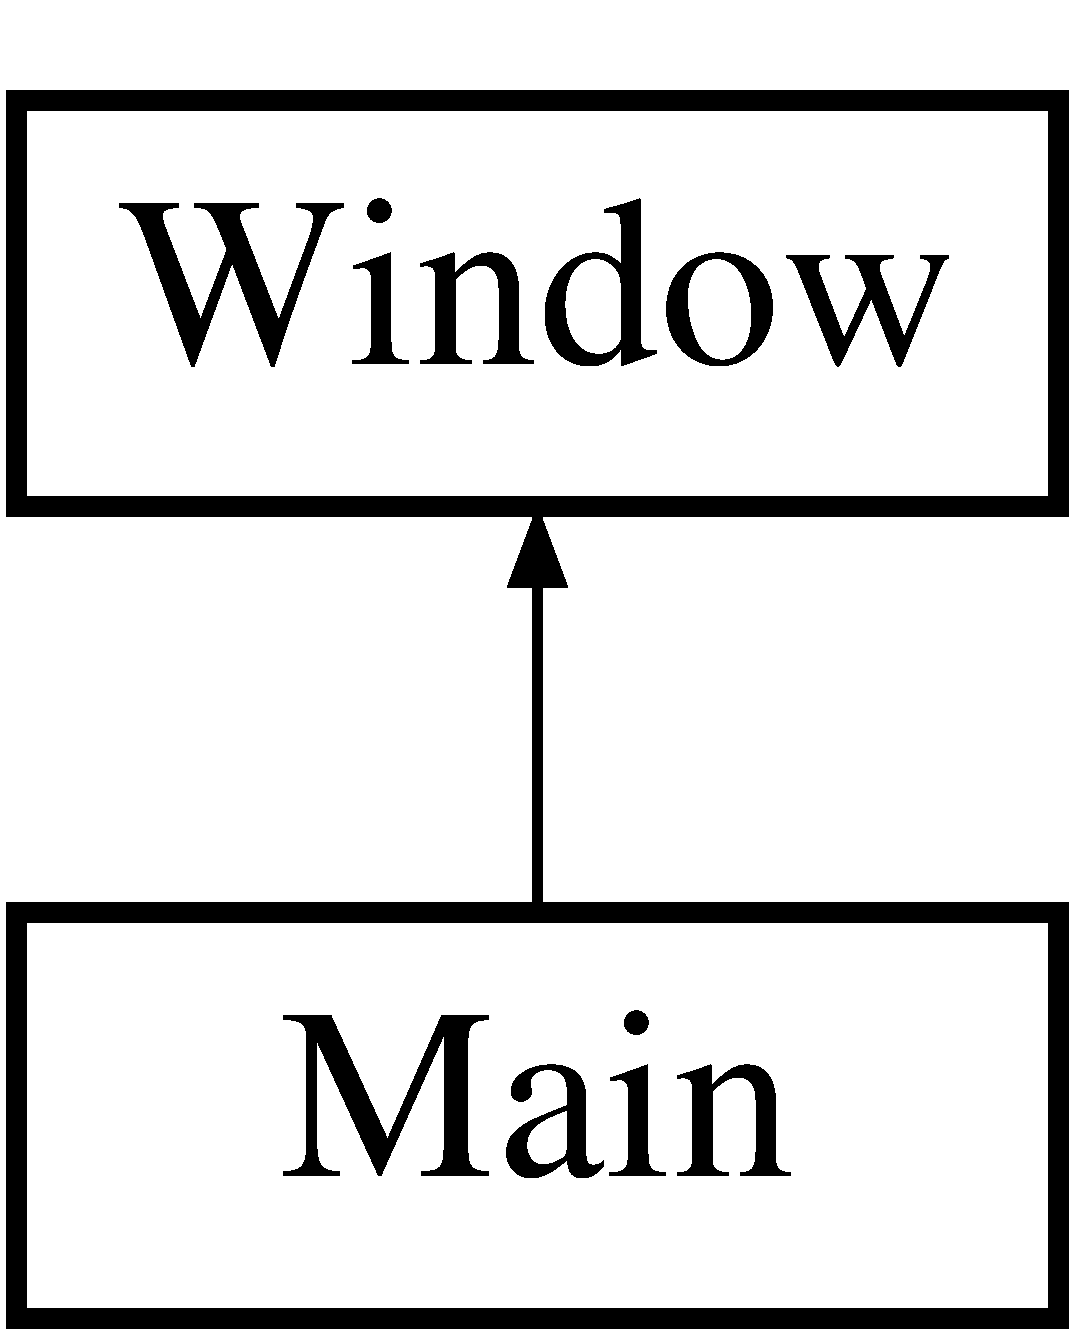
\includegraphics[height=2.000000cm]{class_main}
\end{center}
\end{figure}
\subsection*{Protected Member Functions}
\begin{DoxyCompactItemize}
\item 
\mbox{\Hypertarget{class_main_a81d65a9f5456e36279815ebbfcbedd6e}\label{class_main_a81d65a9f5456e36279815ebbfcbedd6e}} 
void {\bfseries on\+\_\+button\+\_\+clicked1} (Glib\+::ustring data)
\item 
\mbox{\Hypertarget{class_main_a57d500a72d8b963d98ab14aaa1fc8339}\label{class_main_a57d500a72d8b963d98ab14aaa1fc8339}} 
void {\bfseries on\+\_\+button\+\_\+clicked2} (Glib\+::ustring data)
\item 
\mbox{\Hypertarget{class_main_a72a1c6090518a2b17d645099c9fadb34}\label{class_main_a72a1c6090518a2b17d645099c9fadb34}} 
void {\bfseries on\+\_\+button\+\_\+clicked\+\_\+1} (Glib\+::ustring data)
\end{DoxyCompactItemize}
\subsection*{Protected Attributes}
\begin{DoxyCompactItemize}
\item 
\mbox{\Hypertarget{class_main_a58562d3720f7a909016843288d6e86a9}\label{class_main_a58562d3720f7a909016843288d6e86a9}} 
Gtk\+::\+Box {\bfseries m\+\_\+box1}
\item 
\mbox{\Hypertarget{class_main_a0896a22071940aa9da5a47607ee018e1}\label{class_main_a0896a22071940aa9da5a47607ee018e1}} 
Gtk\+::\+Button {\bfseries m\+\_\+button1}
\item 
\mbox{\Hypertarget{class_main_a01ba1b5539c3f65a20bb55e4bbdabcf8}\label{class_main_a01ba1b5539c3f65a20bb55e4bbdabcf8}} 
Gtk\+::\+Button {\bfseries m\+\_\+button2}
\item 
\mbox{\Hypertarget{class_main_a0ac42120551fdc4d4ea7d9c74060e11c}\label{class_main_a0ac42120551fdc4d4ea7d9c74060e11c}} 
Gtk\+::\+Button {\bfseries m\+\_\+button3}
\end{DoxyCompactItemize}


The documentation for this class was generated from the following files\+:\begin{DoxyCompactItemize}
\item 
include/main.\+h\item 
src/helloworld.\+cpp\end{DoxyCompactItemize}

\hypertarget{class_my_area}{}\section{My\+Area Class Reference}
\label{class_my_area}\index{My\+Area@{My\+Area}}
Inheritance diagram for My\+Area\+:\begin{figure}[H]
\begin{center}
\leavevmode
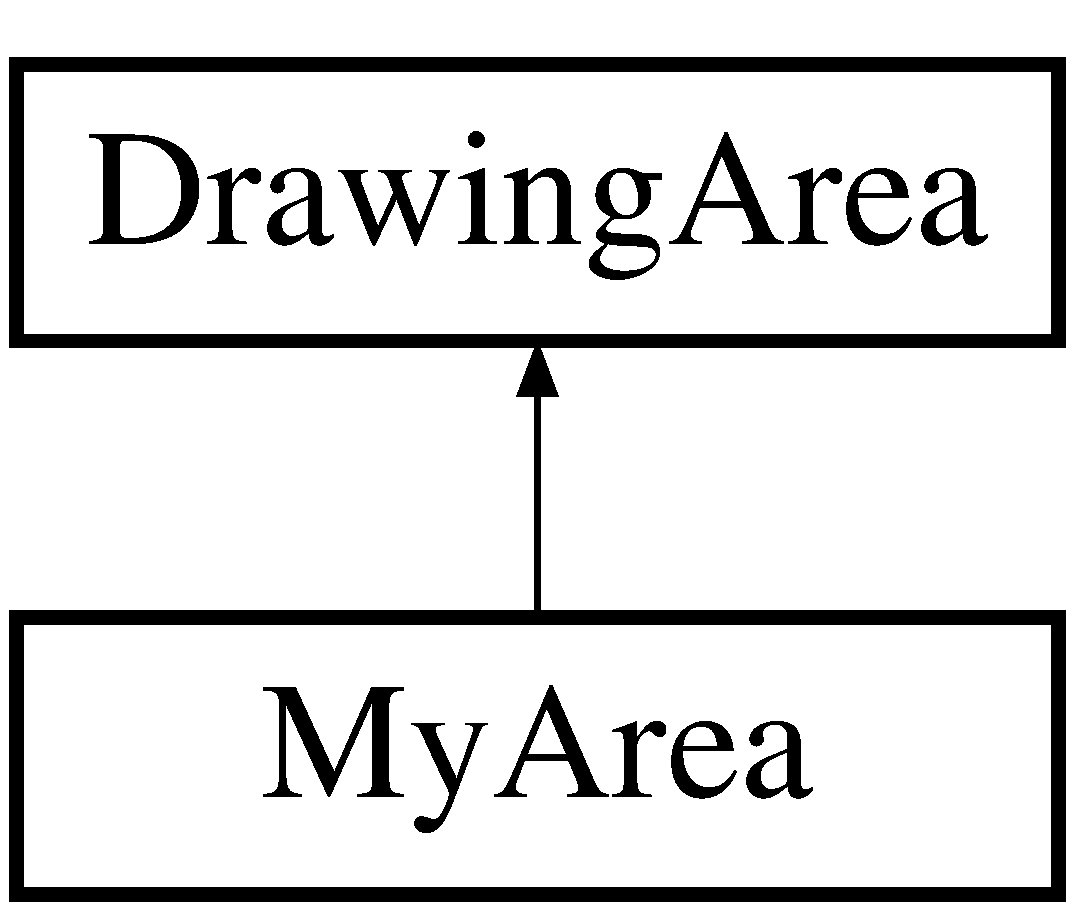
\includegraphics[height=2.000000cm]{class_my_area}
\end{center}
\end{figure}
\subsection*{Public Member Functions}
\begin{DoxyCompactItemize}
\item 
\mbox{\Hypertarget{class_my_area_abfd3125c4ffc88d32742d44e06a13375}\label{class_my_area_abfd3125c4ffc88d32742d44e06a13375}} 
{\bfseries My\+Area} (std\+::string, double, double, double)
\end{DoxyCompactItemize}
\subsection*{Protected Member Functions}
\begin{DoxyCompactItemize}
\item 
bool \mbox{\hyperlink{class_my_area_af5d07988d7c9a6a623ba2fdd3332835b}{on\+\_\+draw}} (const Cairo\+::\+Ref\+Ptr$<$ Cairo\+::\+Context $>$ \&cr) override
\end{DoxyCompactItemize}
\subsection*{Protected Attributes}
\begin{DoxyCompactItemize}
\item 
\mbox{\Hypertarget{class_my_area_a5b95fdb704e973a2e9d4a833d49fe8bd}\label{class_my_area_a5b95fdb704e973a2e9d4a833d49fe8bd}} 
std\+::string {\bfseries file}
\item 
\mbox{\Hypertarget{class_my_area_a32b8946639ee818092a5dce039a48a97}\label{class_my_area_a32b8946639ee818092a5dce039a48a97}} 
double {\bfseries xr}
\item 
\mbox{\Hypertarget{class_my_area_a91dee2e74d98f46ae1d267f5c69cecb5}\label{class_my_area_a91dee2e74d98f46ae1d267f5c69cecb5}} 
double {\bfseries yr}
\item 
\mbox{\Hypertarget{class_my_area_a10a1f8bf97d246395bfe550c0b24aa01}\label{class_my_area_a10a1f8bf97d246395bfe550c0b24aa01}} 
double {\bfseries zr}
\end{DoxyCompactItemize}


\subsection{Member Function Documentation}
\mbox{\Hypertarget{class_my_area_af5d07988d7c9a6a623ba2fdd3332835b}\label{class_my_area_af5d07988d7c9a6a623ba2fdd3332835b}} 
\index{My\+Area@{My\+Area}!on\+\_\+draw@{on\+\_\+draw}}
\index{on\+\_\+draw@{on\+\_\+draw}!My\+Area@{My\+Area}}
\subsubsection{\texorpdfstring{on\+\_\+draw()}{on\_draw()}}
{\footnotesize\ttfamily bool My\+Area\+::on\+\_\+draw (\begin{DoxyParamCaption}\item[{const Cairo\+::\+Ref\+Ptr$<$ Cairo\+::\+Context $>$ \&}]{cr }\end{DoxyParamCaption})\hspace{0.3cm}{\ttfamily [override]}, {\ttfamily [protected]}}

find intersection

find intersection 

The documentation for this class was generated from the following files\+:\begin{DoxyCompactItemize}
\item 
include/myarea.\+h\item 
src/myarea.\+cpp\end{DoxyCompactItemize}

\hypertarget{class_my_area1}{}\section{My\+Area1 Class Reference}
\label{class_my_area1}\index{My\+Area1@{My\+Area1}}
Inheritance diagram for My\+Area1\+:\begin{figure}[H]
\begin{center}
\leavevmode
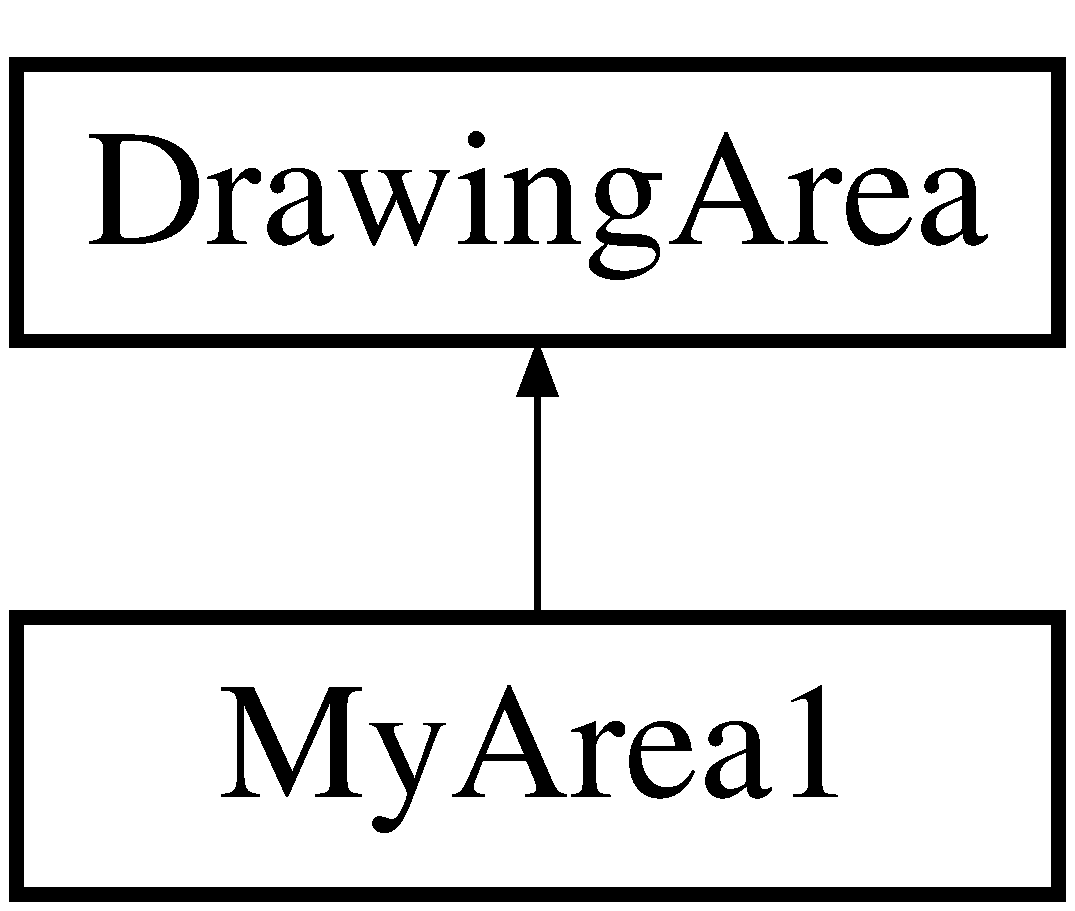
\includegraphics[height=2.000000cm]{class_my_area1}
\end{center}
\end{figure}
\subsection*{Public Member Functions}
\begin{DoxyCompactItemize}
\item 
\mbox{\Hypertarget{class_my_area1_a1fcb3817fdd9f235bf1ac32d00a67e0a}\label{class_my_area1_a1fcb3817fdd9f235bf1ac32d00a67e0a}} 
{\bfseries My\+Area1} (std\+::string, std\+::string, std\+::string)
\end{DoxyCompactItemize}
\subsection*{Protected Member Functions}
\begin{DoxyCompactItemize}
\item 
\mbox{\Hypertarget{class_my_area1_ad8d17dc7c404d0b38135238117824304}\label{class_my_area1_ad8d17dc7c404d0b38135238117824304}} 
bool {\bfseries on\+\_\+timeout} ()
\item 
bool \mbox{\hyperlink{class_my_area1_a0419f61e4d9fc84259fa67cc0dd2a530}{on\+\_\+draw}} (const Cairo\+::\+Ref\+Ptr$<$ Cairo\+::\+Context $>$ \&cr) override
\end{DoxyCompactItemize}
\subsection*{Protected Attributes}
\begin{DoxyCompactItemize}
\item 
\mbox{\Hypertarget{class_my_area1_a77351f73fcbdd228d4ee5b500295c83f}\label{class_my_area1_a77351f73fcbdd228d4ee5b500295c83f}} 
std\+::string {\bfseries file1}
\item 
\mbox{\Hypertarget{class_my_area1_a2fbbd7988cec627660c5bef132eb55c2}\label{class_my_area1_a2fbbd7988cec627660c5bef132eb55c2}} 
std\+::string {\bfseries file2}
\item 
\mbox{\Hypertarget{class_my_area1_a073bac7d92a803fb3b98d0d2ec2a268a}\label{class_my_area1_a073bac7d92a803fb3b98d0d2ec2a268a}} 
std\+::string {\bfseries file3}
\item 
\mbox{\Hypertarget{class_my_area1_abfad1fd0eeb039b67aceef8655aef181}\label{class_my_area1_abfad1fd0eeb039b67aceef8655aef181}} 
double {\bfseries xr}
\item 
\mbox{\Hypertarget{class_my_area1_a5b66572c655d0933edd7a6e7f2395640}\label{class_my_area1_a5b66572c655d0933edd7a6e7f2395640}} 
double {\bfseries yr}
\item 
\mbox{\Hypertarget{class_my_area1_a2b163d39981c522388cc9a2a46e60567}\label{class_my_area1_a2b163d39981c522388cc9a2a46e60567}} 
double {\bfseries zr}
\item 
\mbox{\Hypertarget{class_my_area1_ac3af57e9d8ce69d0a84fce6e7df67829}\label{class_my_area1_ac3af57e9d8ce69d0a84fce6e7df67829}} 
double {\bfseries s}
\item 
\mbox{\Hypertarget{class_my_area1_a40815c991552289013367933373b5751}\label{class_my_area1_a40815c991552289013367933373b5751}} 
double {\bfseries t}
\end{DoxyCompactItemize}


\subsection{Member Function Documentation}
\mbox{\Hypertarget{class_my_area1_a0419f61e4d9fc84259fa67cc0dd2a530}\label{class_my_area1_a0419f61e4d9fc84259fa67cc0dd2a530}} 
\index{My\+Area1@{My\+Area1}!on\+\_\+draw@{on\+\_\+draw}}
\index{on\+\_\+draw@{on\+\_\+draw}!My\+Area1@{My\+Area1}}
\subsubsection{\texorpdfstring{on\+\_\+draw()}{on\_draw()}}
{\footnotesize\ttfamily bool My\+Area1\+::on\+\_\+draw (\begin{DoxyParamCaption}\item[{const Cairo\+::\+Ref\+Ptr$<$ Cairo\+::\+Context $>$ \&}]{cr }\end{DoxyParamCaption})\hspace{0.3cm}{\ttfamily [override]}, {\ttfamily [protected]}}

error

error

check hidden

find intersection

find intersection 

The documentation for this class was generated from the following files\+:\begin{DoxyCompactItemize}
\item 
include/myarea1.\+h\item 
src/myarea1.\+cpp\end{DoxyCompactItemize}

\hypertarget{class_three2}{}\section{Three2 Class Reference}
\label{class_three2}\index{Three2@{Three2}}
Inheritance diagram for Three2\+:\begin{figure}[H]
\begin{center}
\leavevmode
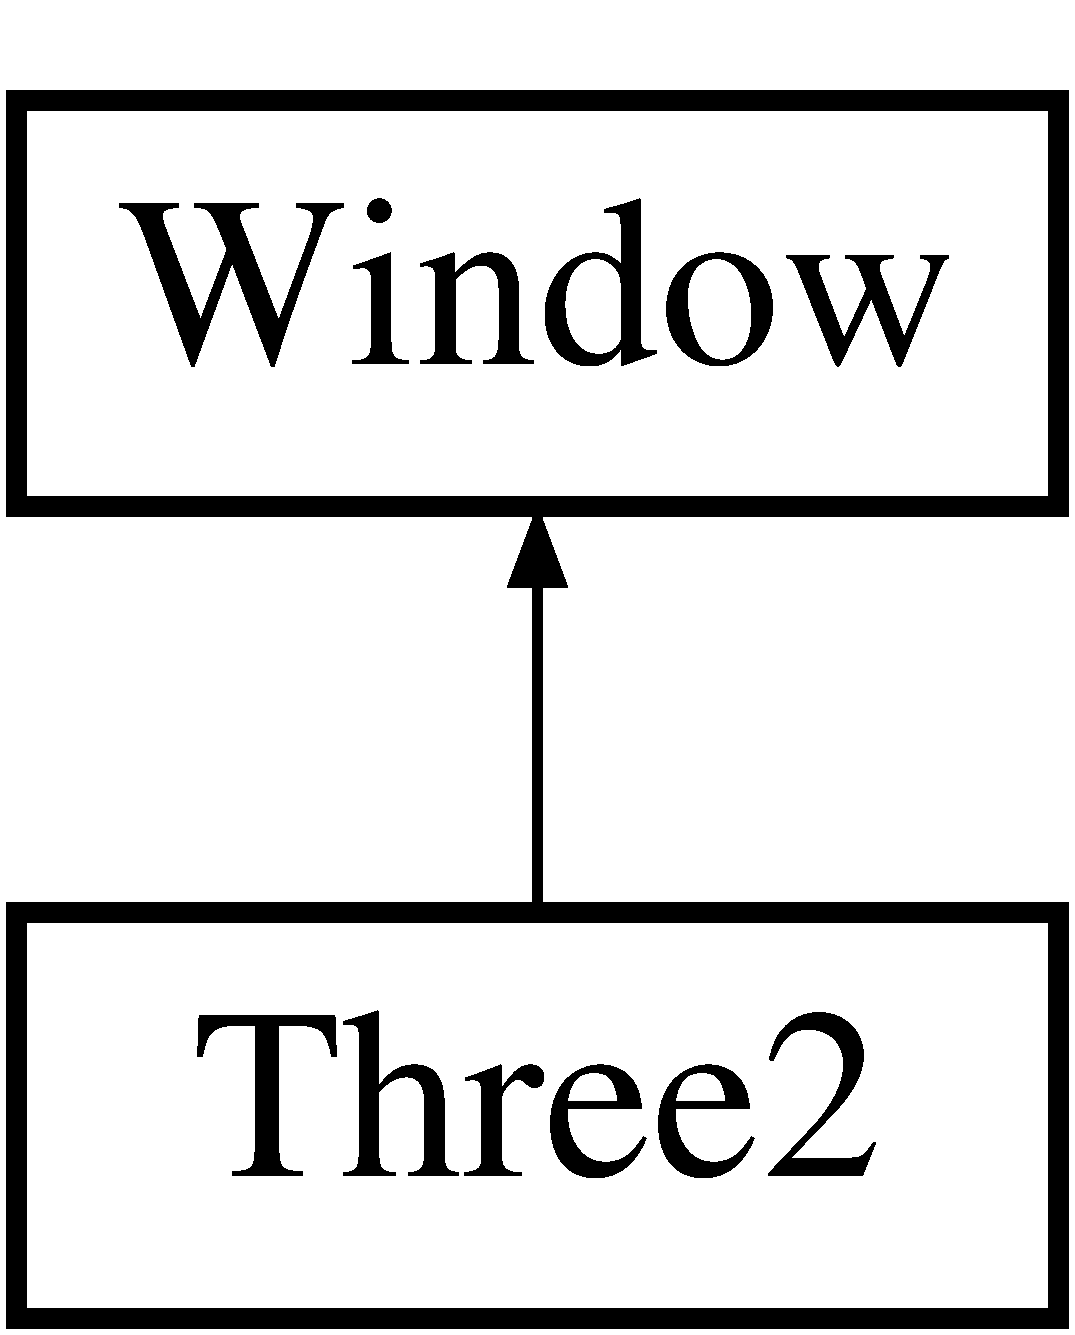
\includegraphics[height=2.000000cm]{class_three2}
\end{center}
\end{figure}
\subsection*{Protected Member Functions}
\begin{DoxyCompactItemize}
\item 
\mbox{\Hypertarget{class_three2_a3a033e3839da176903f784848c7ed3a3}\label{class_three2_a3a033e3839da176903f784848c7ed3a3}} 
void {\bfseries on\+\_\+checkbox\+\_\+editable\+\_\+toggled} ()
\item 
\mbox{\Hypertarget{class_three2_a3bf07f6691f05022993a69ed2c9178dc}\label{class_three2_a3bf07f6691f05022993a69ed2c9178dc}} 
void {\bfseries on\+\_\+checkbox\+\_\+visibility\+\_\+toggled} ()
\item 
\mbox{\Hypertarget{class_three2_a388072d4fa014647e269d63d18ea6d6c}\label{class_three2_a388072d4fa014647e269d63d18ea6d6c}} 
void {\bfseries on\+\_\+button\+\_\+close} ()
\item 
\mbox{\Hypertarget{class_three2_a9140de67b33e78597e81c1714598f9d6}\label{class_three2_a9140de67b33e78597e81c1714598f9d6}} 
void {\bfseries inp} ()
\end{DoxyCompactItemize}
\subsection*{Protected Attributes}
\begin{DoxyCompactItemize}
\item 
\mbox{\Hypertarget{class_three2_adb620701a366dd07844ff4abf17258fe}\label{class_three2_adb620701a366dd07844ff4abf17258fe}} 
std\+::string {\bfseries str}
\item 
\mbox{\Hypertarget{class_three2_aff82a29f9642dc60a115239a0f4cf60b}\label{class_three2_aff82a29f9642dc60a115239a0f4cf60b}} 
Gtk\+::\+Entry {\bfseries m\+\_\+\+Entry\+\_\+x}
\item 
\mbox{\Hypertarget{class_three2_a6b30657ba69e00e4076162e01508ab75}\label{class_three2_a6b30657ba69e00e4076162e01508ab75}} 
Gtk\+::\+Entry {\bfseries m\+\_\+\+Entry\+\_\+y}
\item 
\mbox{\Hypertarget{class_three2_a7d4915ccab1dd3f674cbf456d0fa04bc}\label{class_three2_a7d4915ccab1dd3f674cbf456d0fa04bc}} 
Gtk\+::\+Entry {\bfseries m\+\_\+\+Entry\+\_\+z}
\item 
\mbox{\Hypertarget{class_three2_a96d6bac53e30b6334ebf1cd9cc1e2c32}\label{class_three2_a96d6bac53e30b6334ebf1cd9cc1e2c32}} 
Gtk\+::\+Box {\bfseries m\+\_\+\+H\+Box}
\item 
\mbox{\Hypertarget{class_three2_a9bb049ab7acee838199ca05fdd2a7fd0}\label{class_three2_a9bb049ab7acee838199ca05fdd2a7fd0}} 
Gtk\+::\+Box {\bfseries m\+\_\+\+V\+Box}
\item 
\mbox{\Hypertarget{class_three2_ac424c74203936118ce87aed55c7bce12}\label{class_three2_ac424c74203936118ce87aed55c7bce12}} 
Gtk\+::\+Button {\bfseries m\+\_\+\+Entryx}
\item 
\mbox{\Hypertarget{class_three2_a841fa40683ff4f327693d41c34ad83b5}\label{class_three2_a841fa40683ff4f327693d41c34ad83b5}} 
Gtk\+::\+Button {\bfseries m\+\_\+\+Button\+\_\+\+Close}
\item 
\mbox{\Hypertarget{class_three2_aed3d315fbf91b4cb9c02e5ead67608bc}\label{class_three2_aed3d315fbf91b4cb9c02e5ead67608bc}} 
Gtk\+::\+Button {\bfseries m\+\_\+\+Check\+Button\+\_\+\+Editable}
\item 
\mbox{\Hypertarget{class_three2_af51862b8e6bc0529ca980da25ca19977}\label{class_three2_af51862b8e6bc0529ca980da25ca19977}} 
Gtk\+::\+Button {\bfseries m\+\_\+\+Check\+Button\+\_\+\+Visible}
\end{DoxyCompactItemize}


The documentation for this class was generated from the following files\+:\begin{DoxyCompactItemize}
\item 
include/three2.\+h\item 
src/three2.\+cpp\end{DoxyCompactItemize}

\hypertarget{class_two3}{}\section{Two3 Class Reference}
\label{class_two3}\index{Two3@{Two3}}
Inheritance diagram for Two3\+:\begin{figure}[H]
\begin{center}
\leavevmode
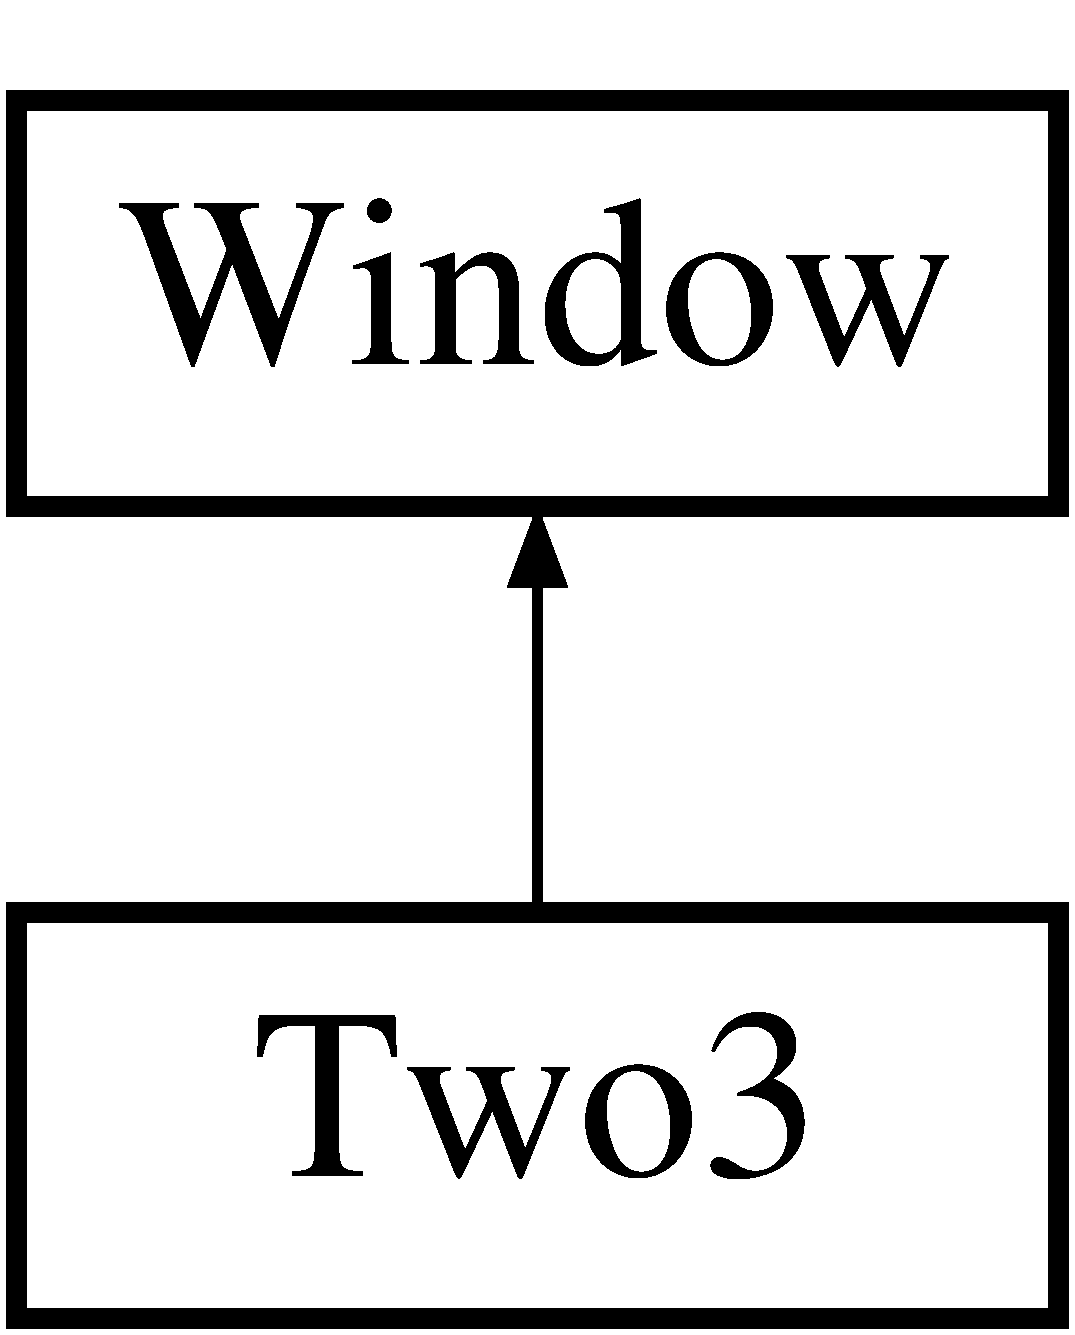
\includegraphics[height=2.000000cm]{class_two3}
\end{center}
\end{figure}
\subsection*{Protected Member Functions}
\begin{DoxyCompactItemize}
\item 
\mbox{\Hypertarget{class_two3_ab375e8888ef602a5f99df24c6795858c}\label{class_two3_ab375e8888ef602a5f99df24c6795858c}} 
void {\bfseries on\+\_\+checkbox\+\_\+editable\+\_\+toggled} ()
\item 
\mbox{\Hypertarget{class_two3_a2552f1956475c6e7534d90abddb08593}\label{class_two3_a2552f1956475c6e7534d90abddb08593}} 
void {\bfseries on\+\_\+checkbox\+\_\+visibility\+\_\+toggled} ()
\item 
\mbox{\Hypertarget{class_two3_a61eecd5981740cc224f6b0d26647eaf0}\label{class_two3_a61eecd5981740cc224f6b0d26647eaf0}} 
void {\bfseries on\+\_\+button\+\_\+close} ()
\item 
\mbox{\Hypertarget{class_two3_adb5d5554ce8ff4d41da0b53239e5cce3}\label{class_two3_adb5d5554ce8ff4d41da0b53239e5cce3}} 
void {\bfseries topview} ()
\item 
\mbox{\Hypertarget{class_two3_a6599c6567169b47d275b5ee4835b3b00}\label{class_two3_a6599c6567169b47d275b5ee4835b3b00}} 
void {\bfseries frontview} ()
\item 
\mbox{\Hypertarget{class_two3_ae834b892a5ad297ab46862026392e919}\label{class_two3_ae834b892a5ad297ab46862026392e919}} 
void {\bfseries sideview} ()
\end{DoxyCompactItemize}
\subsection*{Protected Attributes}
\begin{DoxyCompactItemize}
\item 
\mbox{\Hypertarget{class_two3_a0ef9a390bf346f57853f823da22a2842}\label{class_two3_a0ef9a390bf346f57853f823da22a2842}} 
std\+::string {\bfseries str1}
\item 
\mbox{\Hypertarget{class_two3_af52736463c044343dfdde4d4ef3b5eb4}\label{class_two3_af52736463c044343dfdde4d4ef3b5eb4}} 
std\+::string {\bfseries str2}
\item 
\mbox{\Hypertarget{class_two3_a8c9c9bc6b481aaa5c80293a23464d367}\label{class_two3_a8c9c9bc6b481aaa5c80293a23464d367}} 
std\+::string {\bfseries str3}
\item 
\mbox{\Hypertarget{class_two3_a6f8a95873dfb98bfe64b800dd4d35363}\label{class_two3_a6f8a95873dfb98bfe64b800dd4d35363}} 
Gtk\+::\+Box {\bfseries m\+\_\+\+H\+Box}
\item 
\mbox{\Hypertarget{class_two3_a9b97da6413d7ef432bb8563a294fb035}\label{class_two3_a9b97da6413d7ef432bb8563a294fb035}} 
Gtk\+::\+Box {\bfseries m\+\_\+\+V\+Box}
\item 
\mbox{\Hypertarget{class_two3_aa12311f7070757c39c099b4e4bb0c5cf}\label{class_two3_aa12311f7070757c39c099b4e4bb0c5cf}} 
Gtk\+::\+Button {\bfseries m\+\_\+\+Entryx}
\item 
\mbox{\Hypertarget{class_two3_a4fbd233c33e30ec7c5872d9a7ab40210}\label{class_two3_a4fbd233c33e30ec7c5872d9a7ab40210}} 
Gtk\+::\+Button {\bfseries m\+\_\+\+Entryy}
\item 
\mbox{\Hypertarget{class_two3_ad153f4e4374740fccff887117a6f7bc2}\label{class_two3_ad153f4e4374740fccff887117a6f7bc2}} 
Gtk\+::\+Button {\bfseries m\+\_\+\+Entryz}
\item 
\mbox{\Hypertarget{class_two3_a39c50e6cb6365ada9503a651e21a2fbd}\label{class_two3_a39c50e6cb6365ada9503a651e21a2fbd}} 
Gtk\+::\+Button {\bfseries m\+\_\+\+Button\+\_\+\+Close}
\item 
\mbox{\Hypertarget{class_two3_a0b816fd2d1580adf113c750cb1953aef}\label{class_two3_a0b816fd2d1580adf113c750cb1953aef}} 
Gtk\+::\+Button {\bfseries m\+\_\+\+Check\+Button\+\_\+\+Editable}
\item 
\mbox{\Hypertarget{class_two3_a727573e079e8214ee32836b4fb6b542f}\label{class_two3_a727573e079e8214ee32836b4fb6b542f}} 
Gtk\+::\+Button {\bfseries m\+\_\+\+Check\+Button\+\_\+\+Visible}
\end{DoxyCompactItemize}


The documentation for this class was generated from the following files\+:\begin{DoxyCompactItemize}
\item 
include/two3.\+h\item 
src/two3.\+cpp\end{DoxyCompactItemize}

\hypertarget{classvertex}{}\section{vertex Class Reference}
\label{classvertex}\index{vertex@{vertex}}
\subsection*{Public Member Functions}
\begin{DoxyCompactItemize}
\item 
\mbox{\Hypertarget{classvertex_a18c95e32e1c967b475f39bca2d88073a}\label{classvertex_a18c95e32e1c967b475f39bca2d88073a}} 
{\bfseries vertex} (double xt, double yt, double zt)
\item 
void \mbox{\hyperlink{classvertex_aeee1d0d1d69a140a20e7dd2cd214e616}{rotat}} (double aq, double bq, double cq)
\begin{DoxyCompactList}\small\item\em x,y,z, coordinates of vertex \end{DoxyCompactList}\item 
\mbox{\Hypertarget{classvertex_a72d3b3e034943fb1b1caf1c9ea65a69c}\label{classvertex_a72d3b3e034943fb1b1caf1c9ea65a69c}} 
\mbox{\hyperlink{classvertex}{vertex}} \mbox{\hyperlink{classvertex_a72d3b3e034943fb1b1caf1c9ea65a69c}{cross}} (\mbox{\hyperlink{classvertex}{vertex}} v, \mbox{\hyperlink{classvertex}{vertex}} u)
\begin{DoxyCompactList}\small\item\em To rotate the vertex for 3D to 2D projection. \end{DoxyCompactList}\item 
\mbox{\Hypertarget{classvertex_a9f7b2faefd6156a5d6ebc3115d391433}\label{classvertex_a9f7b2faefd6156a5d6ebc3115d391433}} 
\mbox{\hyperlink{classvertex}{vertex}} {\bfseries sub} (\mbox{\hyperlink{classvertex}{vertex}} v, \mbox{\hyperlink{classvertex}{vertex}} u)
\item 
\mbox{\Hypertarget{classvertex_a5dd8e0928fa7be4dde8701b549769aa8}\label{classvertex_a5dd8e0928fa7be4dde8701b549769aa8}} 
double {\bfseries dot} (\mbox{\hyperlink{classvertex}{vertex}} v)
\end{DoxyCompactItemize}
\subsection*{Public Attributes}
\begin{DoxyCompactItemize}
\item 
\mbox{\Hypertarget{classvertex_a11f52ec2e920d56500baefe5a2e2bba7}\label{classvertex_a11f52ec2e920d56500baefe5a2e2bba7}} 
double {\bfseries x}
\item 
\mbox{\Hypertarget{classvertex_a8b9f211498390a67c369fd43f3722a19}\label{classvertex_a8b9f211498390a67c369fd43f3722a19}} 
double {\bfseries y}
\item 
\mbox{\Hypertarget{classvertex_a4e4f9696a91e9bee75a4c15d8d77e064}\label{classvertex_a4e4f9696a91e9bee75a4c15d8d77e064}} 
double {\bfseries z}
\end{DoxyCompactItemize}


\subsection{Member Function Documentation}
\mbox{\Hypertarget{classvertex_aeee1d0d1d69a140a20e7dd2cd214e616}\label{classvertex_aeee1d0d1d69a140a20e7dd2cd214e616}} 
\index{vertex@{vertex}!rotat@{rotat}}
\index{rotat@{rotat}!vertex@{vertex}}
\subsubsection{\texorpdfstring{rotat()}{rotat()}}
{\footnotesize\ttfamily void vertex\+::rotat (\begin{DoxyParamCaption}\item[{double}]{aq,  }\item[{double}]{bq,  }\item[{double}]{cq }\end{DoxyParamCaption})}



x,y,z, coordinates of vertex 

Normalisation constant

(a,b,c) is unit vector along the perpendicular to the normal

To rotate the vertex 

The documentation for this class was generated from the following files\+:\begin{DoxyCompactItemize}
\item 
include/vertex.\+h\item 
src/vertex.\+cpp\end{DoxyCompactItemize}

%--- End generated contents ---

% Index
\backmatter
\newpage
\phantomsection
\clearemptydoublepage
\addcontentsline{toc}{chapter}{Index}
\printindex

\end{document}
